\documentclass[9pt,a4paper,twocolumn]{article}
\usepackage[margin=1.5cm]{geometry}
\usepackage{graphicx}
\usepackage{booktabs}
\usepackage{amsmath}
\usepackage[hidelinks]{hyperref}
\usepackage{caption}
\captionsetup{font=footnotesize,labelfont=bf,skip=3pt}
\setlength{\parskip}{1.5pt}
\setlength{\parindent}{0pt}
\setlength{\columnsep}{0.65cm}
\pagestyle{empty}

\title{\vspace{-2.2em}GeoMatch: photo geolocation as visual retrieval}
\author{Mohan Manideep Danda}
\date{}

\begin{document}
\maketitle
\vspace{-2.6em}

\begin{figure*}[t]
\centering
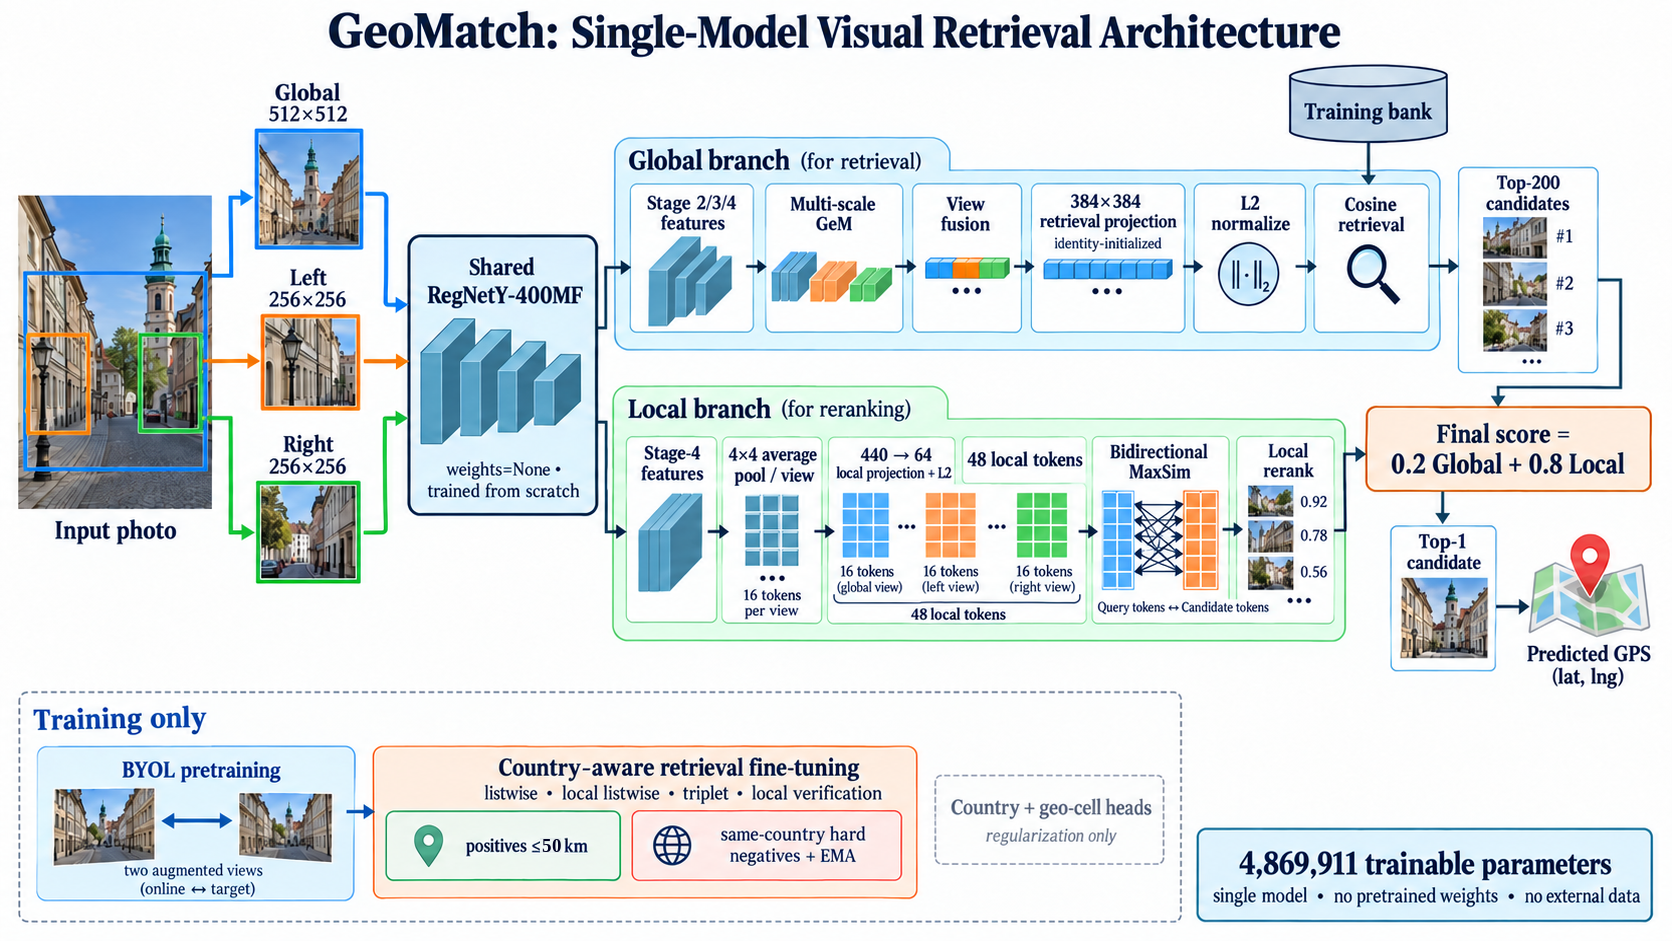
\includegraphics[width=0.95\textwidth]{images/geomatch.png}
\caption{One from-scratch RegNetY-400MF trunk, shared across a global view and
two crops, feeds a global-descriptor retrieval branch and a local-token
late-interaction reranker. The classification heads are a training regulariser
and are not used at inference. $4{,}869{,}911$ parameters.}
\label{fig:arch}
\end{figure*}

\section{Task}

Predict the GPS coordinate of a photo from twelve European countries, scored by
median haversine error. The rules permit \emph{one} model of at most
$5{,}000{,}000$ parameters, no pretrained weights, and no data beyond the
$11{,}758$ labelled training images. Evaluation is on $2{,}400$ held-out photos.

\section{Why retrieval}

The model predicts a location by matching the query against the training set and
copying the coordinate of the best match. This does \emph{not} make the output
continuous --- predictions are restricted to the $11{,}758$ training coordinates,
which is a real quantisation. It is simply a cheap one: the geographically
nearest training photo to a held-out photo is a median of \textbf{3.1\,km} away,
and within 50\,km for \textbf{99.8\%} of queries. That ceiling is an order of
magnitude below the error we actually achieve, so discretisation is not the
binding constraint, whereas a geo-cell classifier is bounded by its cell size.

The real argument for retrieval is that it removes the coordinate regression
problem entirely: the encoder only has to learn \emph{which photos were taken
near each other}, a metric-learning objective that a small from-scratch network
can be supervised on densely, using every pair in a batch.

\section{Model (Fig.~\ref{fig:arch})}

A single RegNetY-400MF trunk (\texttt{weights=None}) is shared across three
views: the full frame at $512^2$ and aligned left/right crops at $256^2$, which
preserve detail that a single downscaled frame destroys.

\textbf{Global branch.} Multi-scale GeM pooling over stages 2--4, fused across
views, through an identity-initialised $384\!\times\!384$ layer, L2-normalised
to a 384-D descriptor $g$.

\textbf{Local branch.} Stage-4 features average-pooled to $4\!\times\!4$ per view
(48 tokens), projected $440\!\to\!64$, L2-normalised to tokens $T$.

For query $q$ and bank image $b$, the shortlist is the cosine top-200 of
$\langle g_q, g_b\rangle$, rescored by a symmetric MaxSim late interaction
\[
s(q,b)=0.2\,\langle g_q,g_b\rangle+0.8\cdot\tfrac12\!\left(
\overline{\max_j}\,T_q T_b^{\!\top} + \overline{\max_i}\,T_q T_b^{\!\top}\right)
\]
where $\overline{\max_j}$ averages the per-token maxima over one axis. The
top-1 candidate's coordinate is the prediction.

\section{Training}

Two stages, evaluated on the official 5-fold split (train four folds, predict the
fifth, fixed epoch count, no checkpoint selection).

\textbf{1. BYOL pretraining} of the trunk (negative-free, momentum target and
predictor), labels unused, 160 epochs.

\textbf{2. Country-aware retrieval fine-tuning}, 40 epochs, AdamW
($8{\times}10^{-5}$ trunk, $6{\times}10^{-4}$ heads), batch 64, EMA 0.999. Each
sampled group is an anchor, two geographic positives ($\le\!50$\,km, drawn by
descriptor similarity from the 64 nearest), and one \emph{same-country} hard
negative $60$--$700$\,km away, mined from the current EMA encoder and refreshed
every epoch. Anchors from the weakest countries are oversampled (DE $3.0\times$,
FR $2.8$, PL $2.0$, IT/ES $1.7$, SE $1.4$, GB $1.3$). The objective is $0.65\,$
retrieval $+\,0.2\,$ classification regulariser; the retrieval term mixes global
listwise/triplet ($0.35$) with local listwise/hinge ($0.65$).

\section{Results}

\begin{table}[h]
\centering\footnotesize
\setlength{\tabcolsep}{4pt}
\begin{tabular}{lccc}
\toprule
pooled 5-fold OOF & $n$ & median (km) & $\le$50\,km \\
\midrule
From-scratch retrieval baseline   & 1 & 89.2 & 45.3\% \\
\;+ BYOL + country-aware, 22 ep   & 1 & 57.7 & 48.8\% \\
\;+ 40 epochs (shipped recipe)    & 3 & \textbf{56.8}\,$\pm$\,1.1 & 48.8\% \\
\midrule
\emph{(non-compliant)} 3-model ensemble & 1 & 52.0 & 49.7\% \\
\emph{(non-compliant)} 6-model ensemble & 1 & 49.7 & 50.1\% \\
\bottomrule
\end{tabular}
\caption{$n$ is the number of independently seeded 5-fold runs. The shipped
recipe's three seeds gave 55.60 / 57.12 / 57.71\,km; we report their mean.
\textbf{Best observed is 55.60\,km}, but that seed was not selected for
submission --- the submitted model uses the config's default seed, which was
never evaluated. Ensembles are listed only to document that the gain is real and
was rejected: the rules require a single ${\le}5$M-parameter model.}
\label{tab:main}
\end{table}

Self-supervised pretraining is the one large win ($-31$\,km). Extending 22 to 40
epochs is within seed noise ($\pm1.1$\,km across three seeds), so we do not claim
it as an improvement; 40 epochs was kept because the schedule was fixed in
advance.

\section{Where the error comes from}

Splitting every query into \emph{located} ($\le$50\,km), \emph{mis-ranked}
(a $\le$50\,km bank image was in the top-200 but not returned first) and
\emph{never retrieved} (no $\le$50\,km image in the top-200) separates the two
failure modes (Fig.~\ref{fig:decomp}).

\begin{table}[h]
\centering\footnotesize
\setlength{\tabcolsep}{5pt}
\begin{tabular}{lccc}
\toprule
& located & mis-ranked & never retrieved \\
\midrule
Pooled  & 49.1\% & 30.3\% & 20.7\% \\
Iceland & 82.9\% & 15.2\% & \phantom{0}1.9\% \\
France  & 25.2\% & 32.7\% & 42.1\% \\
Germany & 14.2\% & 40.6\% & 45.2\% \\
\bottomrule
\end{tabular}
\caption{Ranking is the larger loss pooled, but for Germany and France the
descriptor fails to retrieve any nearby image at all for ${\sim}45\%$ of
queries. Both stages fail there; a better reranker alone could not fix it.}
\label{tab:decomp}
\end{table}

\begin{figure}[h]
\centering
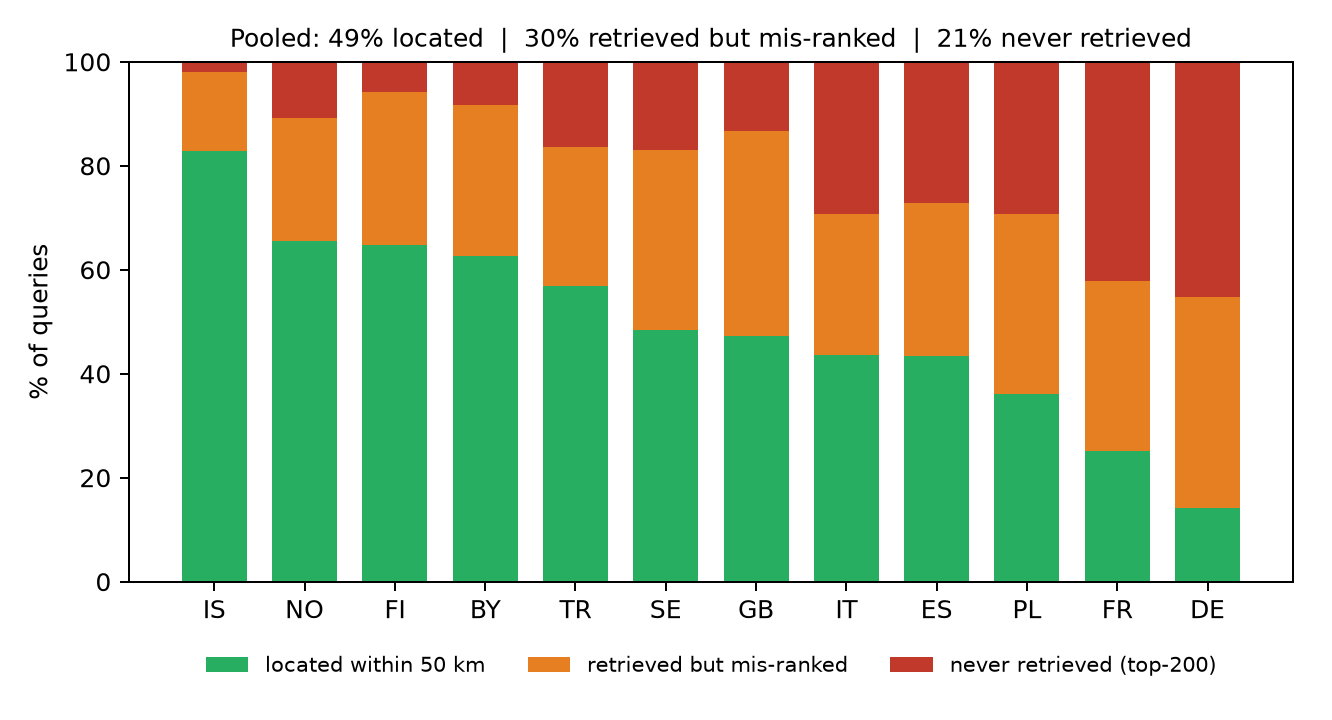
\includegraphics[width=\linewidth]{images/figures/oracle_gap.png}
\caption{Error decomposition per country, sorted by success rate.}
\label{fig:decomp}
\end{figure}

This is why we stopped working on decoding. Germany and France carry the whole
remaining gap (median 505 and 570\,km against ${<}220$\,km everywhere else), and
roughly half of their failures are already lost before any reranking happens.

\section{What did not work}

\textbf{Decode-time repairs on frozen descriptors (5-fold evidence).} A learned
candidate reranker was tried four times (linear, residual, pairwise, and one
gated on a held-out inner fold) and degraded the crossfit every time; the
inner-fold gate passed only because the probe fold was held out from the
reranker but not from the \emph{encoder}. Kernel-density / spatial-consensus
decoding reached 72\,km against 57.7. Restricting the shortlist by predicted
country cost 4\,km pooled (country accuracy is only 68\%, and a wrong gate is
unrecoverable). Decoding from the auxiliary geo-cell head instead of retrieval
gave DE 490 / FR 523\,km against retrieval's 534 / 551 --- equally lost, which is
the strongest evidence that DE/FR location is simply not encoded.

\textbf{Encoder variants (single-fold evidence, weaker).} Adding a
random-resized-crop to the global view was worse at every matched epoch on
fold 0 (e.g.\ 63.7 vs 58.1\,km at epoch 32); it discards the horizon and scene
layout the descriptor needs. Raising the local grid from $4\!\times\!4$ to
$8\!\times\!8$ was \emph{not} clearly worse (58.3 vs 60.7\,km at epoch 40) --- it
is within fold-0 noise, and we kept $4\!\times\!4$ as the simpler option rather
than because the variant failed. Extending that run to 48 epochs drifted back to
61.8\,km. We flag these as suggestive only: the shipped recipe's own fold-0
median wanders between 58.1 and 63.4\,km over epochs 20--40, so single-fold
differences under ${\sim}3$\,km carry no signal.

\section{Limitations}

The dominant one is Germany and France, and the evidence above says it is a
representation failure, not a decoding one: a ${\le}5$M-parameter from-scratch
encoder at 512\,px does not resolve the fine, localised cues (signage, plates,
micro-architecture) that separate suburban scenes repeating over hundreds of
kilometres. Country-aware oversampling and same-country hard negatives target
exactly this and moved every other weak country but not these two. Secondary:
the failed-variant evidence is single-fold; and the figures here are regenerated
from cached out-of-fold predictions that are not checked into the repository.

\section{Submission}

The submitted model is the recipe above retrained once on all $11{,}758$ images
with no held-out fold, initialised from a BYOL trunk, using the configuration's
default seed. It has $4{,}869{,}911$ parameters, trains in $\approx$67\,min on one
RTX 4000 Ada, and writes \texttt{predictions.csv} ($2{,}400$ rows) in
$\approx$5\,min.

\end{document}
